\begin{thm}{108}{\hosi 11}{大数 宿題}
 自然数$n$とし、整数$a, b, c$は、$|a|, |b|, |c| \le n$ を満たす。$x$についての2次方程式 $ax^2+bx+c=0$ が実数解を持つ確率を$p_n$ としたとき、$\disp \lim_{n\to\infty} p_n$ の値を求めよ。
\end{thm}

$-1$以上$n$以下の整数3つの組$(a, b, c)$は全部で$(2n+1)^3$個あるが、そのうち方程式$ax^2+bx+c=0$が実数解を持つものの個数を$W_n$、このうちさらに$a, b\neq 0$を満たすものの個数を$V_n$とおく\footnote{いただいた文献ではこれを$W_n'$としていました。}。
\begin{align*}
 p_n=\frac{W_n}{(2n+1)^3} \,,\,\, V_n\le W_n \le V_n+2(2n+1)^2
\end{align*}
である。$\disp \lim_{n\to\infty} \frac{2(2n+1)^2}{(2n+1)^3}=0$より、はさみうちの原理によって
\[ \lim_{n\to\infty} p_n=\lim_{n\to\infty} \frac{V_n}{(2n+1)^3} \]
となる (ただし右辺の極限値が存在するならば) 。

$a\neq 0$では$ax^2+bx+c=0$は2次方程式であり、これが実数解を持つことは判別式$b^2-4ac$が0以上であることと同値である。$b^2\ge 4ac$かつ$a\neq 0$となる組のうち、$b=k$を満たすものの個数と$b=-k$を満たすものの個数は等しく (ただし$1\le k\le n$)、この値を$S_k$とおけば、$\disp V_n=2\sum_{k=1}^n S_k$となる。

\begin{wrapfigure}[15]{r}[0pt]{120pt}
 \centering
 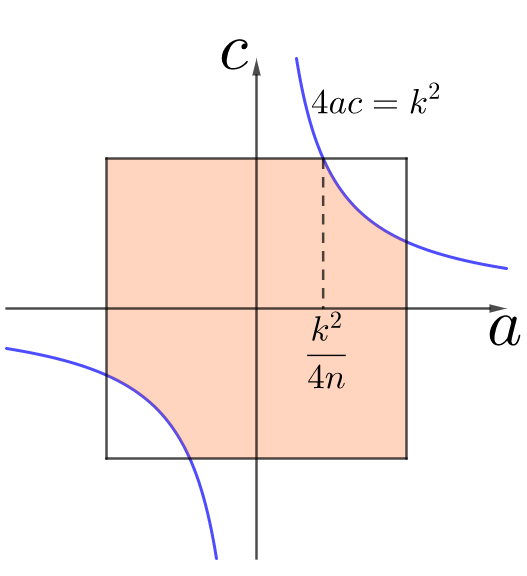
\includegraphics[width=\linewidth]{../problems/Q_108/A_108.png}
\end{wrapfigure}
$S_k$~($1\le k\le n$) は、 $-n\le a, c\le n$, $a\neq 0$, $4ac\le k^2$ を満たす$(a, c)$の組である。このうち$ac\le 0$を満たすものの個数は、$a>0$, $c\le 0$の場合と、$a<0$, $c\ge 0$の場合を数えることで、$2n(n+1)$個とわかる。$ac>0$を満たすものは、$a, c>0$の場合と$a, c<0$の場合に分けられるが、$a, c$の符号を入れ替えることで両者の個数は等しいことがわかる。この値を$T_k$とおけば、
\[ S_k=2T_k+2n(n+1) \]
となる。$1\le a\le \dfrac{k^2}{4n}\,(<n)$のとき、条件を満たす$c$は$c=1, 2, \dots, n$であり、$\dfrac{k^2}{4n}<a\le n$のとき、条件を満たす$c$は$c=1, 2, \dots, \left\lfloor\dfrac{k^2}{4a}\right\rfloor$である。よって、
\[ T_k=\left\lfloor\frac{k^2}{4n}\right\rfloor\cdot n+\sum_{a=\left\lfloor\frac{k^2}{4n}\right\rfloor+1}^n \left\lfloor\frac{k^2}{4n}\right\rfloor \]
となる。これを評価する。第1項については、
\[ \frac{k^2}{4n}-1 \le \left\lfloor\frac{k^2}{4n}\right\rfloor \le \frac{k^2}{4n} \]
であるから、
\[ \frac{k^2}{4}-n \le \left\lfloor\frac{k^2}{4n}\right\rfloor\cdot n\le \frac{k^2}{4} \]
続いて第2項を上から評価する。$a\ge \left\lfloor\dfrac{k^2}{4n}\right\rfloor+2\,(\ge 2)$ のとき、$\dfrac{k^2}{4x}\,(x>0)$が単調減少であることから、
\[ \left\lfloor \frac{k^2}{4a}\right\rfloor \le \frac{k^2}{4a} \le \int_{a-1}^a\! \frac{k^2}{4x} \,dx \]
となるので、
\begin{align*}
 \sum_{a=\left\lfloor\frac{k^2}{4n}\right\rfloor+1}^n \left\lfloor\frac{k^2}{4a}\right\rfloor &\le \sum_{a=\left\lfloor\frac{k^2}{4n}\right\rfloor+2}^n \left\lfloor\frac{k^2}{4a}\right\rfloor + n \\
 &\le \int_{\left\lfloor\frac{k^2}{4n}\right\rfloor+1}^n\frac{k^2}{4x}\,dx + n \le \int_{\frac{k^2}{4n}}^n\frac{k^2}{4x}\,dx + n \\
 &= \frac{k^2}{4}\left(\log n-\log\frac{k^2}{4n}\right)+n = -\frac{k^2}{2}\log\frac{k}{2n}+n
\end{align*}
を得る。次に下から評価する。
\[ \left\lfloor\frac{k^2}{4a}\right\rfloor\ge \frac{k^2}{4a}-1 \ge \int_a^{a+1}\!\frac{k^2}{4x}\,dx -1 \]
であるから、
\begin{align*}
 \sum_{a=\left\lfloor\frac{k^2}{4n}\right\rfloor+1}^n\left\lfloor\frac{k^2}{4a}\right\rfloor &\ge \int_{\left\lfloor\frac{k^2}{4n}\right\rfloor+1}^{n+1}\frac{k^2}{4x}\,dx -n \\
 &=\int_{\frac{k^2}{4n}}^{n+1}\frac{k^2}{4x}\,dx -\int_{\frac{k^2}{4n}}^{\left\lfloor\frac{k^2}{4n}\right\rfloor+1}\frac{k^2}{4x}\,dx -n \\
 &\ge\int_{\frac{k^2}{4n}}^{n+1}\frac{k^2}{4x}\,dx -\int_{\frac{k^2}{4n}}^{\left\lfloor\frac{k^2}{4n}\right\rfloor+1}n\,dx -n \\
 &\ge -\frac{k^2}{2}\log\frac{k}{2n}-2n
\end{align*}
を得る。以上から$T_k$は
\[ \left|T_k-\frac{k^2}{4}\left(1-2\log\frac{k}{2n}\right)\right| \le 3n \]
と評価される。したがって、
\[ V_n=2\sum_{k=1}^nS_k=4\sum_{k=1}^nT_k+4n^2(n+1) \]
であることとあわせて、
\[ \left|V_n-\left(\sum_{k=1}^nk^2\left(1-2\log\frac{k}{2n}\right)+4n^2(n+1)\right)\right| \le 12n^2 \]
を得る。区分求積法により、
\begin{align*}
 &\lim_{n\to\infty}\frac{1}{(2n+1)^3}\sum_{k=1}^nk^2\left(1-2\log\frac{k}{2n}\right) \\
 =& \lim_{n\to\infty}\frac{(2n)^3}{(2n+1)^3}\cdot\frac{1}{2n}\sum_{k=1}^n\left(\frac{k}{2n}\right)^2\left(1-2\log\frac{k}{2n}\right) \\
 =& \int_0^{\frac{1}{2}}\! x^2(1-2\log x) \,dx \\
 =& \Bigl[\frac{x^3}{3}(1-2\log x)\Bigr]^{\frac{1}{2}}_0-\int_0^{\frac{1}{2}}\frac{x^3}{3}\left(-\frac{2}{x}\right) \,dx \\
 =& \Bigl[\frac{x^3}{3}\left(\frac{5}{3}-2\log x\right)\Bigr]^{\frac{1}{2}}_0 = \frac{1}{24}\left(\frac{5}{3}+2\log 2\right)=\frac{5}{72}+\frac{\log 2}{12}
\end{align*}
と求まる\footnote{ここで$x^2\log x$や$x^3\log x$は$x=0$において0となるものとして計算している。こう定義しておけば$x\ge 0$において連続な関数になる。}。続いて $\disp \lim_{n\to\infty}\frac{4n^2(n+1)}{(2n+1)^3}=\frac{1}{2}$ である。

最後に$\disp \lim_{n\to\infty}\frac{12n^2}{(2n+1)^3}=0$ であるからはさみうちの原理が適用できて、
\[ \lim_{n\to\infty}p_n=\lim_{n\to\infty}\frac{V_n}{(2n+1)^3}=\left(\frac{5}{72}+\frac{\log 2}{12}\right)+\frac{1}{2}=\frac{41}{72}+\frac{\log 2}{12} \]